% !TEX TS-program = XeLaTeX
% use the following command:
% all document files must be coded in UTF-8
\documentclass[portuguese]{textolivre}
% build HTML with: make4ht -e build.lua -c textolivre.cfg -x -u article "fn-in,svg,pic-align"

\journalname{Texto Livre}
\thevolume{19}
%\thenumber{1} % old template
\theyear{2026}
\receiveddate{\DTMdisplaydate{2026}{10}{17}{-1}} % YYYY MM DD
\accepteddate{\DTMdisplaydate{2026}{10}{19}{-1}}
\publisheddate{\DTMdisplaydate{2026}{10}{26}{-1}}
\corrauthor{Mariah dos Santos}
\articledoi{10.1590/1983-3652.2026.69219}
%\articleid{NNNN} % if the article ID is not the last 5 numbers of its DOI, provide it using \articleid{} commmand 
% list of available sesscions in the journal: articles, dossier, reports, essays, reviews, interviews, editorial
\articlesessionname{reviews}
\runningauthor{Santos} 
%\editorname{Leonardo Araújo} % old template
\sectioneditorname{Daniervelin Pereira~\orcid{0000-0003-1861-3609}}
\layouteditorname{Leonardo Araújo~\orcid{0000-0003-3884-2177}}

\title{Resenha do livro Escrever e ensinar a escrever: breve antimanual para docentes}
\othertitle{Review of Escrever e ensinar a escrever: breve antimanual para docentes}
% if there is a third language title, add here:
%\othertitle{Artikelvorlage zur Einreichung beim Texto Livre Journal}

\author[1]{Mariah dos Santos~\orcid{0009-0001-5451-3608}\thanks{Email: \href{mailto:mariah.santos2580@gmail.com}{mariah.santos2580@gmail.com}}}
\affil[1]{Universidade de Minas Gerais, Faculdade de Letras, Belo Horizonte, MG, Brasil.}

\addbibresource{article.bib}
% use biber instead of bibtex
% $ biber article

% used to create dummy text for the template file
\definecolor{dark-gray}{gray}{0.35} % color used to display dummy texts
\usepackage{lipsum}
\SetLipsumParListSurrounders{\colorlet{oldcolor}{.}\color{dark-gray}}{\color{oldcolor}}

% used here only to provide the XeLaTeX and BibTeX logos
\usepackage{hologo}

% if you use multirows in a table, include the multirow package
\usepackage{multirow}

% provides sidewaysfigure environment
\usepackage{rotating}

\usepackage{endnotes} % Inclui o pacote endnotes

% CUSTOM EPIGRAPH - BEGIN 
%%% https://tex.stackexchange.com/questions/193178/specific-epigraph-style
\usepackage{epigraph}
\renewcommand\textflush{flushright}
\makeatletter
\newlength\epitextskip
\pretocmd{\@epitext}{\em}{}{}
\apptocmd{\@epitext}{\em}{}{}
\patchcmd{\epigraph}{\@epitext{#1}\\}{\@epitext{#1}\\[\epitextskip]}{}{}
\makeatother
\setlength\epigraphrule{0pt}
\setlength\epitextskip{0.5ex}
\setlength\epigraphwidth{.7\textwidth}
% CUSTOM EPIGRAPH - END

% to use IPA symbols in unicode add
%\usepackage{fontspec}
%\newfontfamily\ipafont{CMU Serif}
%\newcommand{\ipa}[1]{{\ipafont #1}}
% and in the text you may use the \ipa{...} command passing the symbols in unicode

% LANGUAGE - BEGIN
% ARABIC
% for languages that use special fonts, you must provide the typeface that will be used
% \setotherlanguage{arabic}
% \newfontfamily\arabicfont[Script=Arabic]{Amiri}
% \newfontfamily\arabicfontsf[Script=Arabic]{Amiri}
% \newfontfamily\arabicfonttt[Script=Arabic]{Amiri}
%
% in the article, to add arabic text use: \textlang{arabic}{ ... }
%
% RUSSIAN
% for russian text we also need to define fonts with support for Cyrillic script
% \usepackage{fontspec}
% \setotherlanguage{russian}
% \newfontfamily\cyrillicfont{Times New Roman}
% \newfontfamily\cyrillicfontsf{Times New Roman}[Script=Cyrillic]
% \newfontfamily\cyrillicfonttt{Times New Roman}[Script=Cyrillic]
%
% in the text use \begin{russian} ... \end{russian}
% LANGUAGE - END

% EMOJIS - BEGIN
% to use emoticons in your manuscript
% https://stackoverflow.com/questions/190145/how-to-insert-emoticons-in-latex/57076064
% using font Symbola, which has full support
% the font may be downloaded at:
% https://dn-works.com/ufas/
% add to preamble:
% \newfontfamily\Symbola{Symbola}
% in the text use:
% {\Symbola }
% EMOJIS - END

% LABEL REFERENCE TO DESCRIPTIVE LIST - BEGIN
% reference itens in a descriptive list using their labels instead of numbers
% insert the code below in the preambule:
%\makeatletter
%\let\orgdescriptionlabel\descriptionlabel
%\renewcommand*{\descriptionlabel}[1]{%
%  \let\orglabel\label
%  \let\label\@gobble
%  \phantomsection
%  \edef\@currentlabel{#1\unskip}%
%  \let\label\orglabel
%  \orgdescriptionlabel{#1}%
%}
%\makeatother
%
% in your document, use as illustraded here:
%\begin{description}
%  \item[first\label{itm1}] this is only an example;
%  % ...  add more items
%\end{description}
% LABEL REFERENCE TO DESCRIPTIVE LIST - END


% add line numbers for submission
%\usepackage{lineno}
%\linenumbers

\begin{document}
\maketitle

\begin{figure}[htbp]
\centering
\begin{minipage}{.5\textwidth}
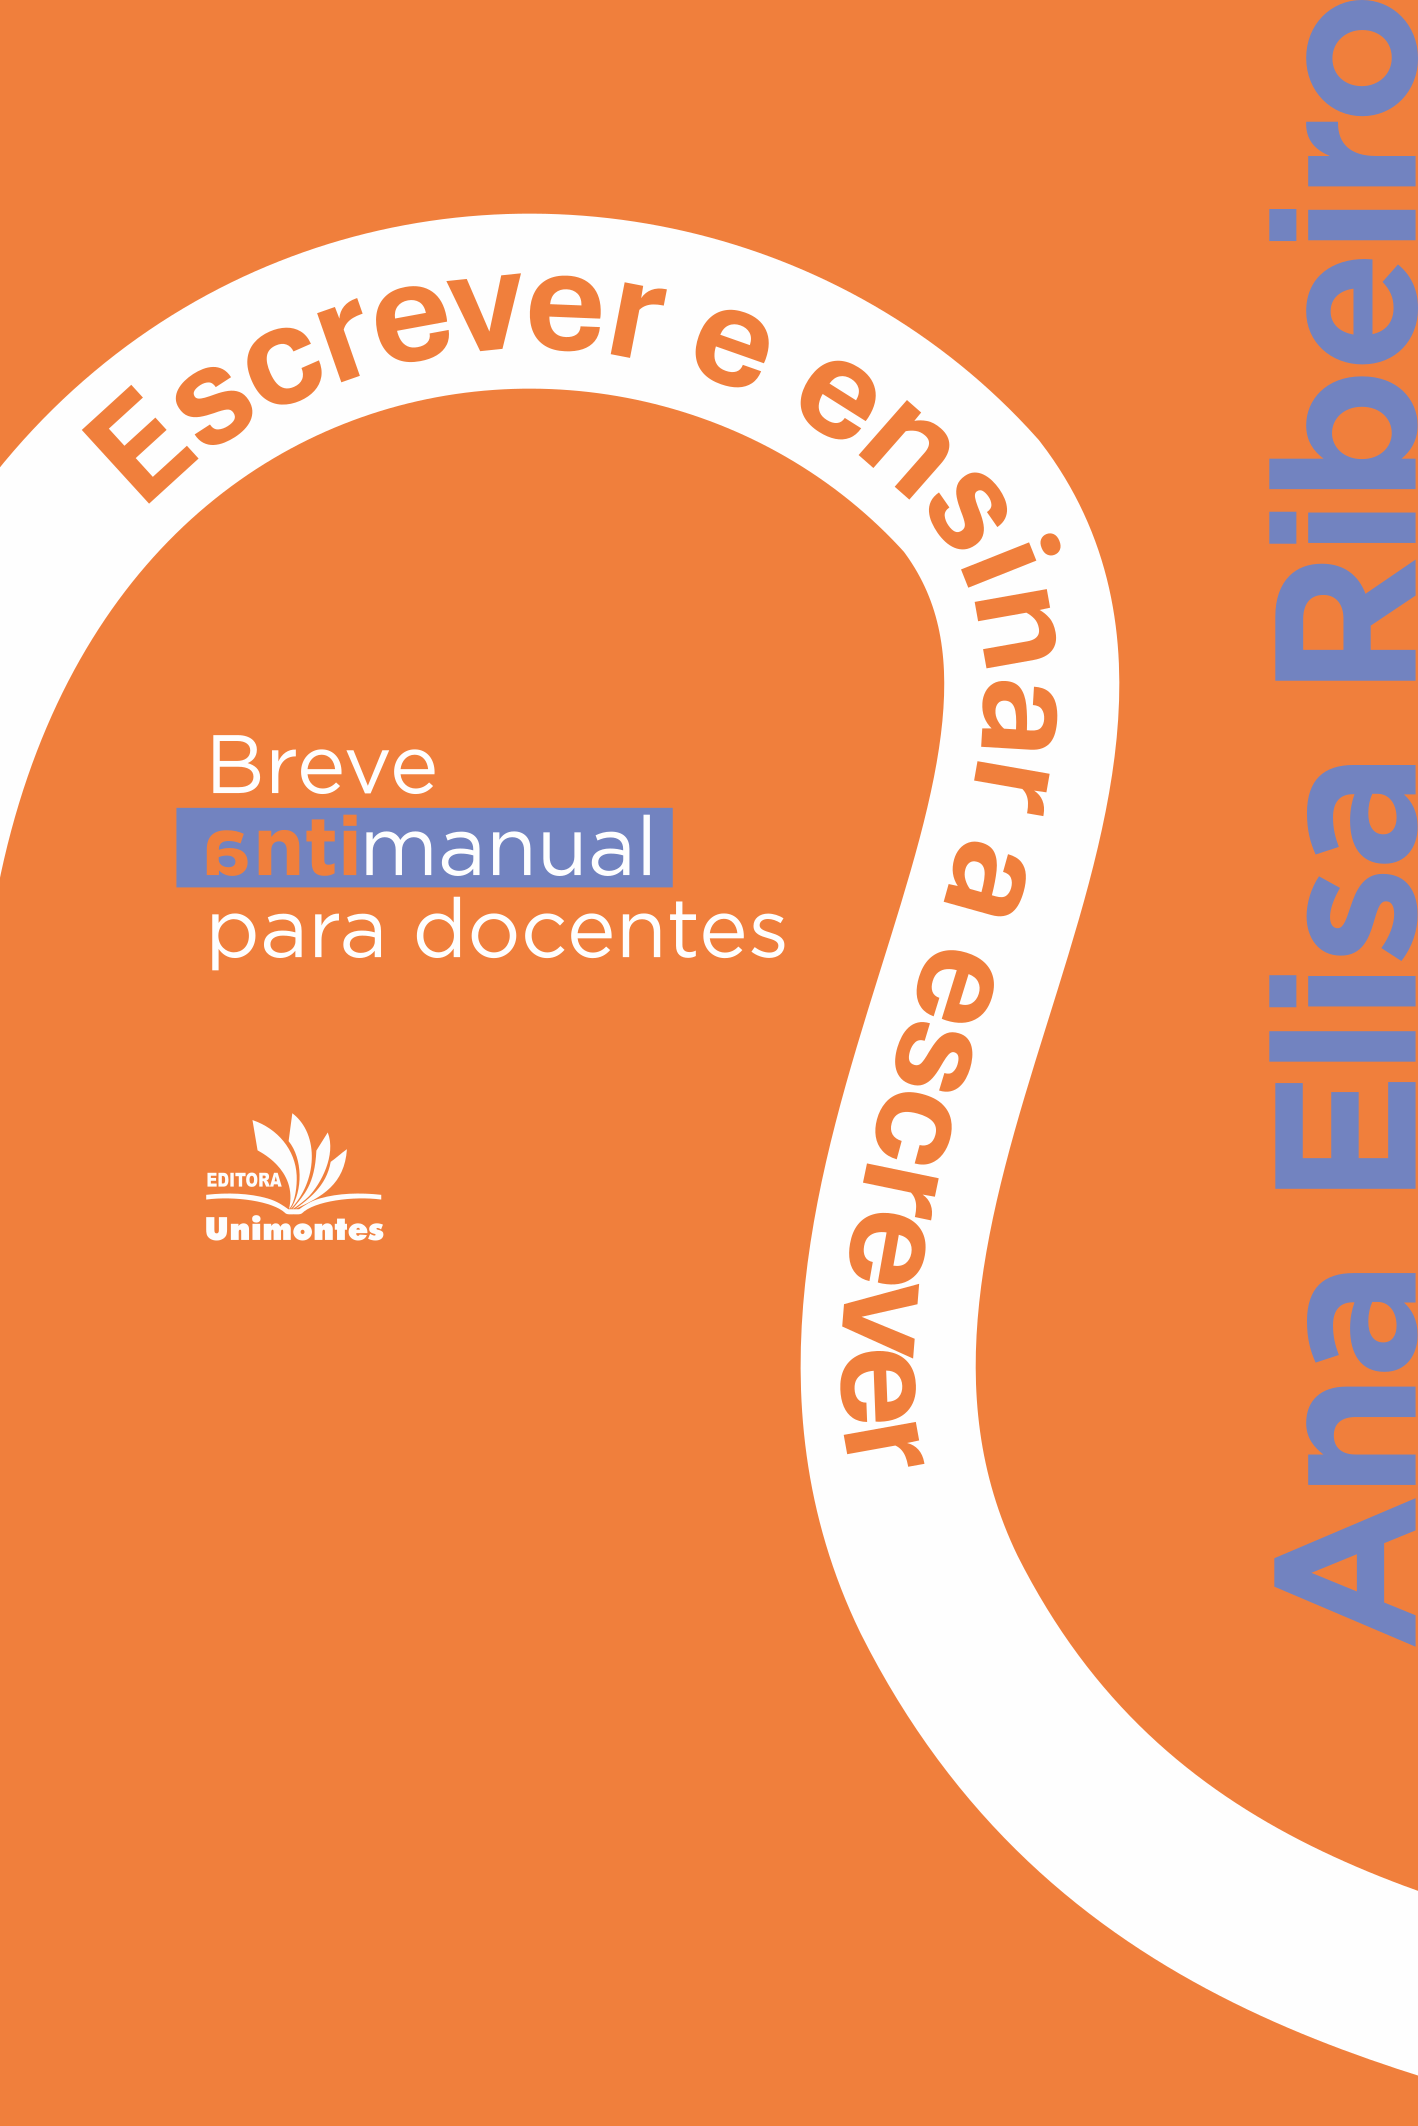
\includegraphics[width=\textwidth]{Fig1.png}
 \caption*{\fullcite{ribeiro2025escrever}}
 \label{fig01}
\end{minipage}
\end{figure}

\begin{polyabstract}
\begin{abstract}
Esta resenha apresenta e discute o livro \citetitle{ribeiro2025escrever}, de Ana Elisa Ribeiro, publicado em 2025 pela Editora Unimontes em acesso aberto. A obra reúne quatro textos curtos e um apêndice que tratam da correção e do comentário de textos na escola, da proposta ENA (estranhar, nomear e ajustar), da revisão de textos literários e do uso da inteligência artificial na escrita e na correção de redações. A resenha descreve cada capítulo e destaca a coerência entre a forma do livro e a tese que ele defende. Também aponta limites: a distância entre a proposta da autora e as condições da maioria das escolas públicas, o deslocamento do capítulo sobre revisão editorial, as repetições próprias de uma coletânea e a falta de referências precisas para algumas ideias de outros autores. Conclui que a obra é recomendada a professores de língua portuguesa, estudantes de Letras e revisores, mas não a quem procura um manual com roteiros prontos.

\keywords{Ensino de escrita \sep Correção de textos \sep Revisão de textos \sep Inteligência Artificial \sep Linguística Aplicada}
\end{abstract}

\begin{english}
\begin{abstract}
This review presents and discusses \citetitle{ribeiro2025escrever}, by Ana Elisa Ribeiro, published in 2025 by Editora Unimontes as an open-access work. The book brings together four short texts and an appendix addressing the correction and commentary of school texts, the ENA approach (estranhar, nomear e ajustar [defamiliarize, name, and adjust]), the revision of literary texts, and the use of artificial intelligence in writing and essay assessment. The review describes each chapter and highlights the coherence between the book’s form and the thesis it advances. It also identifies several limitations: the gap between the author’s proposal and the conditions prevailing in most public schools, the inclusion of a chapter on editorial revision that seems somewhat out of place, repetitions inherent in a collection of texts, and the lack of precise references for some ideas attributed to other authors. The review concludes that the book is recommended for Portuguese language teachers, language and literature students, and proofreaders and editors, but not for readers seeking a manual with ready-made procedures.

\keywords{Writing instruction \sep Text correction \sep Text revision \sep Artificial Intelligence \sep Applied Linguistics}
\end{abstract}
\end{english}
% if there is another abstract, insert it here using the same scheme
\end{polyabstract}

Há uma cena no segundo texto do livro \citetitle{ribeiro2025escrever} que resume bem o problema discutido nele. Uma aluna entrega um conto e pergunta: “Professora, você vai corrigir nossos contos?” \cite[p.~23]{ribeiro2025escrever}. A professora titubeia. Não quer dizer que não, mas também não quer dizer que sim, porque o que ela pretende fazer não é corrigir: é comentar. A pergunta parece banal e não é. Ela carrega a suposição de que o texto já nasceu errado e de que consertá-lo é tarefa de outra pessoa.

Escrever e ensinar a escrever: breve antimanual para docentes saiu em 2025 pela Editora da Unimontes, em tiragem impressa distribuída a escolas públicas e em PDF de acesso aberto. São 87 páginas que reúnem quatro textos curtos. Três já haviam circulado entre 2022 e 2023, no blog da Parábola Editorial e na Revista Ponte; o quarto, sobre inteligência artificial, é inédito. Fecham o volume um apêndice — a fala que a autora preparou para uma audiência pública sobre ChatGPT na Assembleia Legislativa de Minas Gerais, em julho de 2023 — e uma lista de leituras que ela batiza de “Referências livres”. A obra foi selecionada por edital de divulgação científica e passou por parecer duplo cego, o que ajuda a explicar seu tom: apoiada em estudos da Linguística Aplicada, mas escrita para ser lida fora dos congressos.

Ana Elisa Ribeiro é doutora em Linguística Aplicada pela UFMG e professora titular do CEFET-MG, onde atua no ensino médio integrado, na graduação em Letras (Tecnologias da Edição) e na pós-graduação em Estudos de Linguagens. Também escreve literatura e trabalha há anos como revisora no mercado editorial. Essa condição tripla — professora de Redação, pesquisadora e revisora — sustenta o livro inteiro, e a autora a usa como argumento mais de uma vez. O propósito está declarado logo na nota inicial: chegar “ao coração de colegas que atuam nas escolas ou no ensino de escrita” \cite[p.~11]{ribeiro2025escrever}. O prefixo do título é um aviso ao leitor. Quem procurar sequência didática pronta, modelo de rubrica ou lista de macetes vai fechar o livro frustrado.

O primeiro texto, “3 passos – firmes – rumo ao escrever na escola”, é o mais próximo de uma proposta operacional. Ribeiro descreve três movimentos que persegue com suas turmas ao longo do ano e resume na sigla ENA: estranhar a própria escrita, nomear o que está estranho e ajustar o texto. O estranhamento que interessa não é o do professor experiente, e sim o do próprio estudante, aquele desconfiômetro que diz “tem uma coisa esquisita neste trecho” \cite[p.~16]{ribeiro2025escrever}. Antes de chegar aos três passos, a autora enfileira uma pequena tipologia das devolutivas que circulam nas escolas: correções-rabiscos, correções-humilhação, correções-código-indecifrável, correções-escribas, entre outras \cite[p.~15-16]{ribeiro2025escrever}. A lista é curta e desconcertante, porque qualquer pessoa que passou pela educação básica reconhece ali pelo menos duas.

O segundo texto, “Por que não gosto de corrigir textos”, desenvolve a cena da aluna e o conto. Ribeiro separa duas atividades que costumam ser confundidas. Como revisora, ela resolve: o livro chega com problemas, ela conserta e quase nunca precisa explicar por quê. Como professora, resolver é justamente o que ela não quer fazer, porque a tarefa ali é ensinar. Chama atenção que esse recuo não venha acompanhado de nenhum abandono da gramática. A autora conta que pergunta às alunas onde está o sujeito da oração antes de discutir a vírgula, e observa que, sem esse conhecimento, o comentário sobre pontuação não significa nada para elas. A descrição da língua continua necessária, defende \textcite[p.~28]{ribeiro2025escrever}, mas é preciso “tomá-las para dançar”. O fechamento do capítulo é mais duro do que o resto: ensinar a escrever, na escola regular, seria uma tarefa quase impossível, sabotada pelo currículo, pelo relógio e pela quantidade de papéis \cite[p.~29]{ribeiro2025escrever}.

O terceiro texto, “Uma mirada rebelde sobre a revisão de textos”, muda de cenário e vai para o mercado editorial. A autora discute o que chama de materiais rebeldes: poemas, contos, romances e livros infantis que pedem do revisor uma leitura contextualizada, e não a aplicação automática da norma. O melhor exemplo é o de um livro infantil em que uma bruxa, numa conversa informal com um menino, responde “vire-se”. A forma obedece à regra que proíbe começar oração com pronome oblíquo e destrói a verossimilhança da fala, já que em português brasileiro ninguém diz isso: diz-se “se vira”. Para \textcite[p.~37]{ribeiro2025escrever}, o texto ganha em correção e perde em expressão. Ela também trata da diferença entre revisar autores mortos e vivos, e de casos-limite, como o de um escritor contemporâneo que publica em “portunhol selvagem”. Ao fim, transfere a pergunta para a escola: com que parâmetros comentamos os poemas e as crônicas dos nossos alunos?

O quarto texto, “Devemos temer a inteligência artificial?”, é o mais longo e o mais atual. Ribeiro parte de uma explicação simples do funcionamento de ferramentas como o ChatGPT: não há pensamento nem senciência, há cálculo de probabilidade sobre um banco imenso de textos, muito maior em inglês do que em português. Ela critica o que chama de metáforas fofas — inteligência, nuvem, alucinação —, que, no seu argumento, escondem o mecanismo e criam um imaginário equivocado sobre a máquina \cite[p.~50]{ribeiro2025escrever}. A parte mais interessante do capítulo trata da correção automática de redações em massa, que já foi adotada por redes estaduais. O raciocínio da autora é incômodo e bem construído: se a grade é clara, se o texto tem fórmula e se há um corpus grande de redações, então a máquina realmente faz o serviço, e faz mais rápido. O problema, então, não estaria na ferramenta, e sim no modelo de escrita que a tornou substituível. Convidada a comentar o assunto na televisão, ela resumiu a posição em uma frase: quem precisa melhorar a escrita é o estudante, não a ferramenta \cite[p.~53]{ribeiro2025escrever}. O apêndice retoma esse debate em outro registro e traz um episódio saboroso: ao pedir ao ChatGPT informações sobre a própria vida de escritora, Ribeiro recebeu um texto bem redigido e cheio de erros, com livros que ela nunca escreveu. “Mas eu sei disso. E quem não sabe?” \cite[p.~81]{ribeiro2025escrever}.

Parece-me que o livro cumpre o que promete, e cumpre principalmente por causa de uma coerência que nem sempre aparece em obras sobre ensino de escrita: a forma do texto pratica a tese que ele defende. Um volume que argumenta a favor da interlocução, da intenção e do direito à rebeldia não poderia ser escrito em prosa acadêmica engessada. Ribeiro escreve em primeira pessoa, abre os capítulos com cenas de sala de aula, deixa perguntas sem resposta e usa humor. O resultado é um texto que se lê em uma tarde e que, ainda assim, não simplifica o que discute. A sigla ENA merece destaque à parte, porque é o tipo de ferramenta que um professor consegue levar para a aula seguinte sem precisar de formação continuada, material novo ou autorização da coordenação.

Há, no entanto, um ponto que me parece frágil, e ele é o mesmo em quase todos os capítulos. A autora escreve de um lugar bastante particular. Ela própria descreve o CEFET-MG como um espaço em que se sente livre e autônoma como profissional \cite[p.~23]{ribeiro2025escrever} e menciona aulas de redação semanais, em formato de oficina, com tempo para reescrita e discussão coletiva. Essa é a condição que torna o ENA possível. O livro reconhece a precariedade da escola pública com honestidade — fala em centenas de meios papéis escritos às pressas, em dois textos por ano, em retornos silenciosos —, mas o diagnóstico e a proposta não chegam a se encontrar. Faltou, a meu ver, um capítulo que traduzisse os três passos para a professora com cinco turmas de quarenta alunos. Sem isso, corre-se o risco de que o antimanual seja lido, exatamente pelo público que ele quer alcançar, como um retrato do que seria bonito fazer em outra escola.

Uma segunda ressalva diz respeito ao terceiro texto. Ele é o mais bem escrito do conjunto e também o mais deslocado. As discussões sobre revisão de autores vivos e mortos, sobre capital simbólico e sobre a relação entre revisor e editor interessam a quem trabalha com edição, e a ponte com a sala de aula fica concentrada em perguntas rápidas, quase todas no fim das seções. Uma professora de português encontrará ali uma boa provocação sobre hipercorreção, mas pouco material para transformar em aula. Já a organização do volume como coletânea cobra seu preço: como os textos nasceram separados, a defesa do comentário no lugar da correção reaparece três vezes, e o argumento sobre a fórmula do Enem é praticamente repetido entre o quarto capítulo e o apêndice. A própria autora avisa que os textos são desdobramentos uns dos outros, o que atenua a crítica sem eliminá-la para quem lê o livro de ponta a ponta.

Resta um comentário de ordem metodológica, importante para o leitor que pretenda usar a obra em pesquisa. A opção pelas “Referências livres” é coerente com o projeto de divulgação científica, e a autora explica que muitas de suas leituras estão difusas no texto. O efeito, porém, é que ideias alheias aparecem sem indicação precisa de origem. Mary Kalantzis e Bill Cope são apresentados como referência central da discussão sobre letramento e inteligência artificial, e a expressão “letramento ciber-social” chega ao leitor em tradução livre da própria autora, sem página. Roberto Casati, Jan Masschelein e Maarten Simons são convocados no apêndice do mesmo modo. Quem quiser citar essas formulações precisará ir aos originais, e não ao antimanual. Trata-se de uma escolha legítima para o gênero, não de um descuido, mas convém que o leitor iniciante saiba disso antes de transformar o livro em referencial teórico.

A leitura vale a pena e é recomendada, em primeiro lugar, a professoras e professores de língua materna da educação básica, sobretudo aos que lidam com produção de textos no ensino médio e andam desconfortáveis com a caneta vermelha. Serve muito bem, também, a estudantes de Letras em formação inicial, pelo desenho realista do que é ensinar a escrever no Brasil, e a revisores de texto interessados na dimensão ética do ofício. Coordenadores e gestores que estejam avaliando a compra de sistemas de correção automática de redações deveriam ler pelo menos o quarto capítulo antes de assinar qualquer contrato. Não recomendo o livro, por outro lado, a quem procura um manual: não há roteiro de aula, não há rubrica de avaliação, não há modelo replicável, e essa ausência é deliberada. Também encontrará pouco quem espere uma condenação simples das tecnologias digitais, porque a posição da autora vai na direção oposta. Não deveríamos temer as inteligências artificiais, escreve \textcite[p.~65]{ribeiro2025escrever}; deveríamos compreender como funcionam, para que sejamos nós a decidir o que fazer com elas. Em oitenta e sete páginas de acesso aberto, é um convite difícil de recusar.



\printbibliography\label{sec-bib}
% if the text is not in Portuguese, it might be necessary to use the code below instead to print the correct ABNT abbreviations [s.n.], [s.l.]
%\begin{portuguese}
%\printbibliography[title={Bibliography}]
%\end{portuguese}

\section*{\fontsize{10}{12}\selectfont Agradecimentos}
Agradeço à professora Daniervelin Renata Marques Pereira e à professora Ana Elisa Ribeiro pelo incentivo e pela oportunidade de submeter este trabalho.

\begin{dataavailability}
\txtdataavailability{nodata} % options: dataavailable, dataonly, databody, datanotav, nodata
\end{dataavailability}

\end{document}

